\documentclass[a4paper,12pt]{report}
\usepackage[utf8]{inputenc}
\usepackage[francais]{babel}
\usepackage{fancyhdr}
\usepackage{graphicx}
\usepackage{tikz}
\usetikzlibrary{arrows}
\usetikzlibrary{calc}
\definecolor{grey}{rgb}{0.9,0.9,0.9}
\usepackage{titlesec}
\usepackage{listings}
\usepackage{textcomp}
\usepackage{hyperref}
\usepackage{ amssymb }
\usepackage{xcolor}
\usepackage{listings}
\usepackage{amsmath}
\lstset{basicstyle=\ttfamily,
  showstringspaces=false,
  commentstyle=\color{red},
  keywordstyle=\color{blue}
}

\frenchbsetup{StandardLists=true}
\newcommand{\marge}{18mm}
\usepackage[left=\marge,right=\marge,top=\marge,bottom=\marge]{geometry}
\pagestyle{fancy}
\setlength{\headheight}{14pt}
\chead{
  \textbf{Binome :} Douaille Erwan $\&$ Miranda Yoan
  \hspace{2em}
  \textbf{Groupe :} M1 Info groupe 4}
\renewcommand{\headrulewidth}{0pt}
\linespread{1.3}
\setlength{\columnseprule}{0.2pt}

\usetikzlibrary{matrix,arrows,decorations.pathmorphing}

\begin{document}
\section*{README}

Le code non symétrique se trouve dans nosym.c\\
Le code symétrique se trouve dans sym.c\\
Le code de la q10 se trouve dans jeuAlgo.c\\
\begin{lstlisting}[language=bash]
./jeuAlgo 10 7 7 3
\end{lstlisting}

\section*{Question 1}
\begin{tikzpicture}[->,>=stealth',shorten >=1pt,auto,node distance=3cm,
  thick,main node/.style={circle,fill=blue!20,draw,font=\sffamily\Large\bfseries}]

  \node[main node] (1) {+3};
  \node[main node] (2) [below left of=1] {+1};
  \node[main node] (3) [below right of=2] {+1};
  \node[main node] (4) [below right of=1] {-2};
  \node[main node] (5) [below right of=4] {+1};
  \node[main node] (6) [below of=3] {0};

  \path[every node/.style={font=\sffamily\small}]
    (1) edge [right] node[left] {} (2)
    		edge [left] node[right] {} (4)
    		edge [bend left] node[left] {} (5)
    (2) edge node [right] {} (6)
   		edge [left] node[right] {} (3)
    (3) edge node [right] {} (6)
    (4) edge [right] node[left] {} (3)
    		edge [left] node[right] {} (5)
    (5) edge node [right] {} (6);
\end{tikzpicture}

\section*{Question 2}
(max(nb negatif)-1)*-(1), et, (max(nb)+1)*(-1)
%\begin{figure}[!ht]
	%\center
	%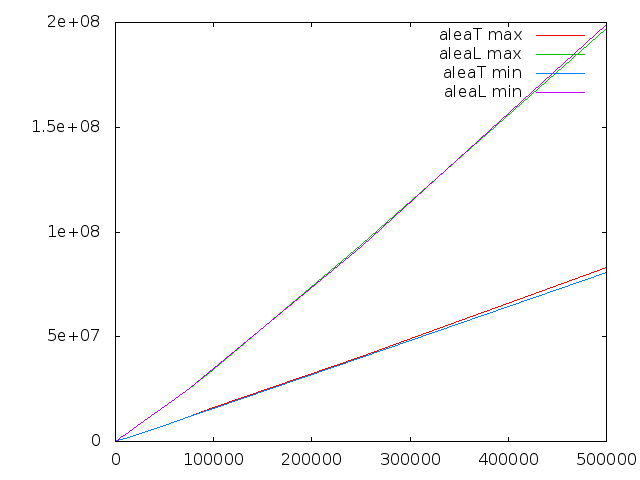
\includegraphics[scale=0.5]{q1.png}
	%\caption{les temps d’execution des methodes aleaL et aleaT}
%\end{figure}

\section*{Question 3}
\begin{itemize}
	\item 10 7 7 3: 1 secondes (moins de 1 seconde)
	\item 10 7 5 3: 1 secondes (moins de 1 seconde)
\end{itemize}

\section*{Question 4}
\begin{itemize}
	\item 100 100 50 50: -198
	\item 100 100 48 52: 191
\end{itemize}

\newpage

\section*{Question 5}
\begin{lstlisting}[language=bash]
wawan@wawan-fixe:~/Dropbox/Master/AAC/tp2$ ./jeuAlgo
conf a 127 pour un tablau 127*127:0 63 
conf a 127 pour un tablau 127*127:63 0 
conf a 127 pour un tablau 127*127:63 126 
conf a 127 pour un tablau 127*127:126 63 
\end{lstlisting}

\section*{Question 6}
(m\up{2} * n\up{2})

\section*{Question 7}
Ces configurations ont la même valeur car ce sont les même. Imaginons que notre tablette de chocolat est une matrice à 2 dimensions (et c'est le cas), il suffit d'appliquer des transformations dessus pour obtenir les autres tablettes. Voici un exemple de transformation qui peut-être appliqué:

\[
M=
  \begin{bmatrix}
    1 & 2 & 3 & 4 \\
    1 & 2 & 3 & 4 \\
    1 & 2 & 3 & 4 \\
    1 & 2 & 3 & 4 \\
  \end{bmatrix} x
  \begin{bmatrix}
    0 & 0 & 0 & 1 \\
    0 & 0 & 1 & 0 \\
    0 & 1 & 0 & 0 \\
    1 & 0 & 0 & 0 \\
  \end{bmatrix} =
  \begin{bmatrix}
    4 & 3 & 2 & 1 \\
    4 & 3 & 2 & 1 \\
    4 & 3 & 2 & 1 \\
    4 & 3 & 2 & 1 \\
  \end{bmatrix}
\]
La version simplifiée consiste juste à dire que la tablette a subit des rotations, des inversions ...

\section*{Question 8}

Avec la symétrie le résultat est 6 fois plus rapide.
Non symétrique: 
\begin{itemize}
\item configuration coup -198 Duree = 7s
\item configuration coup 191 Duree = 8s
\end{itemize}
Symétrique: 
\begin{itemize}
\item configuration coup -198 Duree = 1s
\item configuration coup 191 Duree = 1s
\end{itemize}

\section*{Question 9}

Je ne l'ai pas écrit dans mon code mais le principe est de faire en sorte que le carré de la mort soit toujours en haut à gauche pour économiser des calculs grâce à la symétrie.

\section*{Question 10}
Faite, il suffit de lancer ./jeuAlgo 10 7 5 3, par exemple.

\end{document}